\begin{table}[htbp]\centering\small
\begin{tabular}{llrrrrrr}
\toprule
model & economy & weights & \shortstack{corr with\\truth} & \shortstack{corr,\\MLP fit} & \shortstack{nonlinear\\share} & \shortstack{corr of non-\\linear parts ($t$)} & \shortstack{interaction\\sd at pair} \\
\midrule
BGN & \texttt{bgnbase} (benchmark; size $\times$ bm) & true SDF & 1.00 & 0.77 & 0.35 &  & 0.076 \\
 &  & FMR & 0.43 & 0.57 & 0.11 & +0.28 (89.4) & 0.012 \\
 &  & FF & 0.35 & 0.44 & 0.35 & +0.11 (6.8) & 0.039 \\
 &  & DKKM & 0.45 & 0.60 & 0.04 & +0.37 (4.9) & 0.008 \\
\midrule
BGN & \texttt{bvych0} (3b; size $\times$ bm) & true SDF & 1.00 & 0.38 & 0.39 &  & 0.051 \\
 &  & FMR & 0.17 & 0.21 & 0.07 & +0.00 (0.4) & 0.013 \\
 &  & FF & 0.19 & 0.24 & 0.17 & +0.19 (14.2) & 0.019 \\
 &  & DKKM & 0.24 & 0.24 & 0.03 & +0.49 (59.9) & 0.013 \\
\midrule
GS21 & \texttt{gsbase} (benchmark; bm $\times$ roe) & true SDF & 1.00 & 0.97 & 0.11 &  & 0.004 \\
 &  & FMR & 0.54 & 0.74 & 0.07 & +0.13 (14.3) & 0.002 \\
 &  & FF & 0.48 & 0.69 & 0.39 & +0.30 (21.7) & 0.002 \\
 &  & DKKM & 0.57 & 0.79 & 0.14 & -0.12 (-8.3) & 0.000 \\
\midrule
GS21 & \texttt{gvyp10} (3b; bm $\times$ roe) & true SDF & 1.00 & 0.98 & 0.50 &  & 0.052 \\
 &  & FMR & 0.25 & 0.28 & 0.16 & +0.61 (68.8) & 0.021 \\
 &  & FF & 0.40 & 0.40 & 0.16 & +0.33 (17.8) & 0.025 \\
 &  & DKKM & 0.83 & 0.86 & 0.38 & +0.84 (83.9) & 0.033 \\
\midrule
KP14 & \texttt{kpbase} (benchmark; size $\times$ bm) & true SDF & 1.00 & 0.80 & 0.08 &  & 0.008 \\
 &  & FMR & 0.37 & 0.59 & 0.10 & +0.02 (1.4) & 0.006 \\
 &  & FF & 0.31 & 0.42 & 0.20 & +0.24 (17.3) & 0.016 \\
 &  & DKKM & 0.33 & 0.41 & 0.10 & -0.10 (-23.5) & 0.009 \\
\midrule
KP14 & \texttt{vyg25} (3b; size $\times$ bm) & true SDF & 1.00 & 0.67 & 0.58 &  & 0.112 \\
 &  & FMR & 0.29 & 0.33 & 0.19 & -0.13 (-18.2) & 0.012 \\
 &  & FF & 0.35 & 0.39 & 0.33 & +0.18 (16.6) & 0.095 \\
 &  & DKKM & 0.48 & 0.55 & 0.21 & +0.77 (229.0) & 0.110 \\
\bottomrule
\end{tabular}
\caption{Neural-network fits of the portfolio weights: benchmark and group-3b economies.}\label{tab:mlp}
\begin{minipage}{\textwidth}\footnotesize Columns: corr with truth = mean over (seed, month) cross-sections of the correlation between the method's weights and the true SDF weights; corr, MLP fit = the same for the MLP surface fitted to the method's weights; nonlinear share = the part of the fitted surface's variance that an OLS fit on the five ranks within each cross-section leaves (one minus the within-cross-section $R^2$); corr of nonlinear parts = cross-sectional correlation of that nonlinear remainder with the truth surface's nonlinear remainder, with its t-statistic across seeds; interaction sd at pair = standard deviation, in weight units, of the two-way interaction part of the fitted surface over the named pair (the surface minus its additive fit in the two characteristics), so the truth's row says how large the interaction is and a method's row how much of it the method's weights carry. The pair is the one the economy's exposure is written in (KP14 and BGN: type, proxied by size, times leverage, bm; GS21: productivity, roe, times leverage, bm) and is the pair the figures use. Seeds: three per benchmark, ten per 3b economy; evaluation months only; DKKM at $P=3600$ and the economy's best $\kappa$; weights winsorized at 1/99 within cross-sections.\end{minipage}
\end{table}
\begin{figure}[htbp]\centering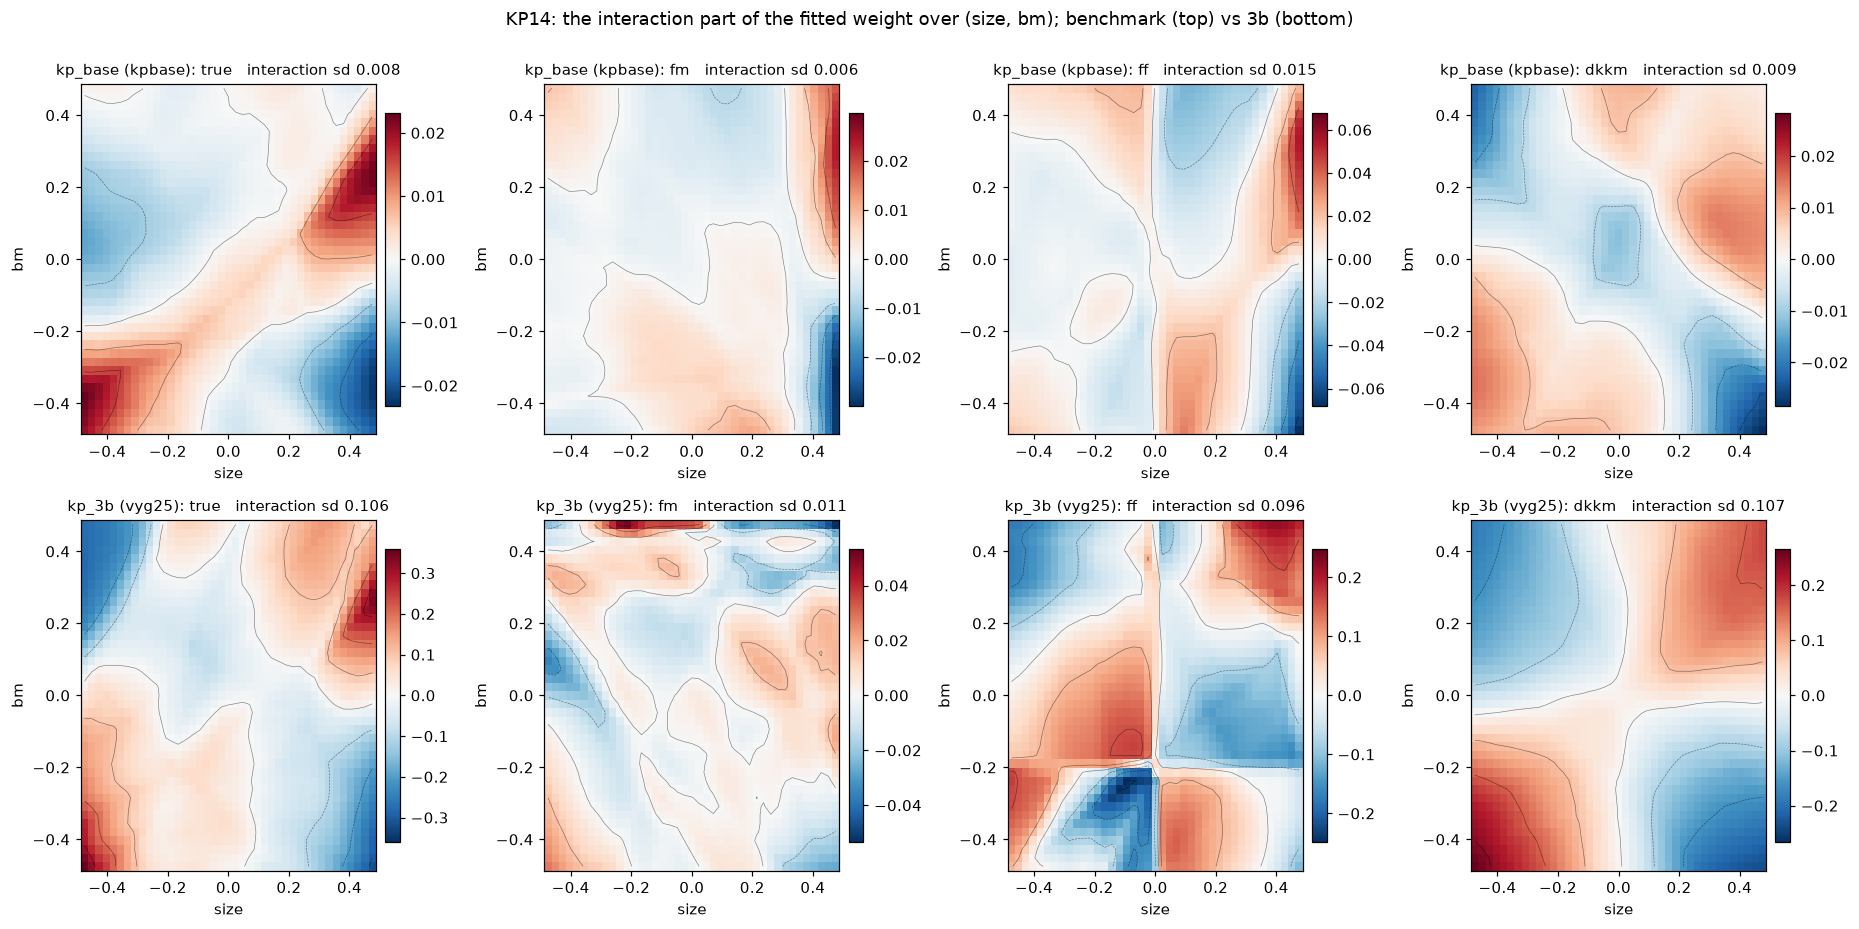
\includegraphics[width=\textwidth]{mlp_figures/interaction_kp_sizexbm.png}\caption{KP14: the interaction part of the fitted weight over book-to-market and size (benchmark above, 3b below); panels: true SDF, Fama--MacBeth, Fama--French, DKKM, each on its own colour scale, the interaction's sd in weight units in the title.}\end{figure}
\begin{figure}[htbp]\centering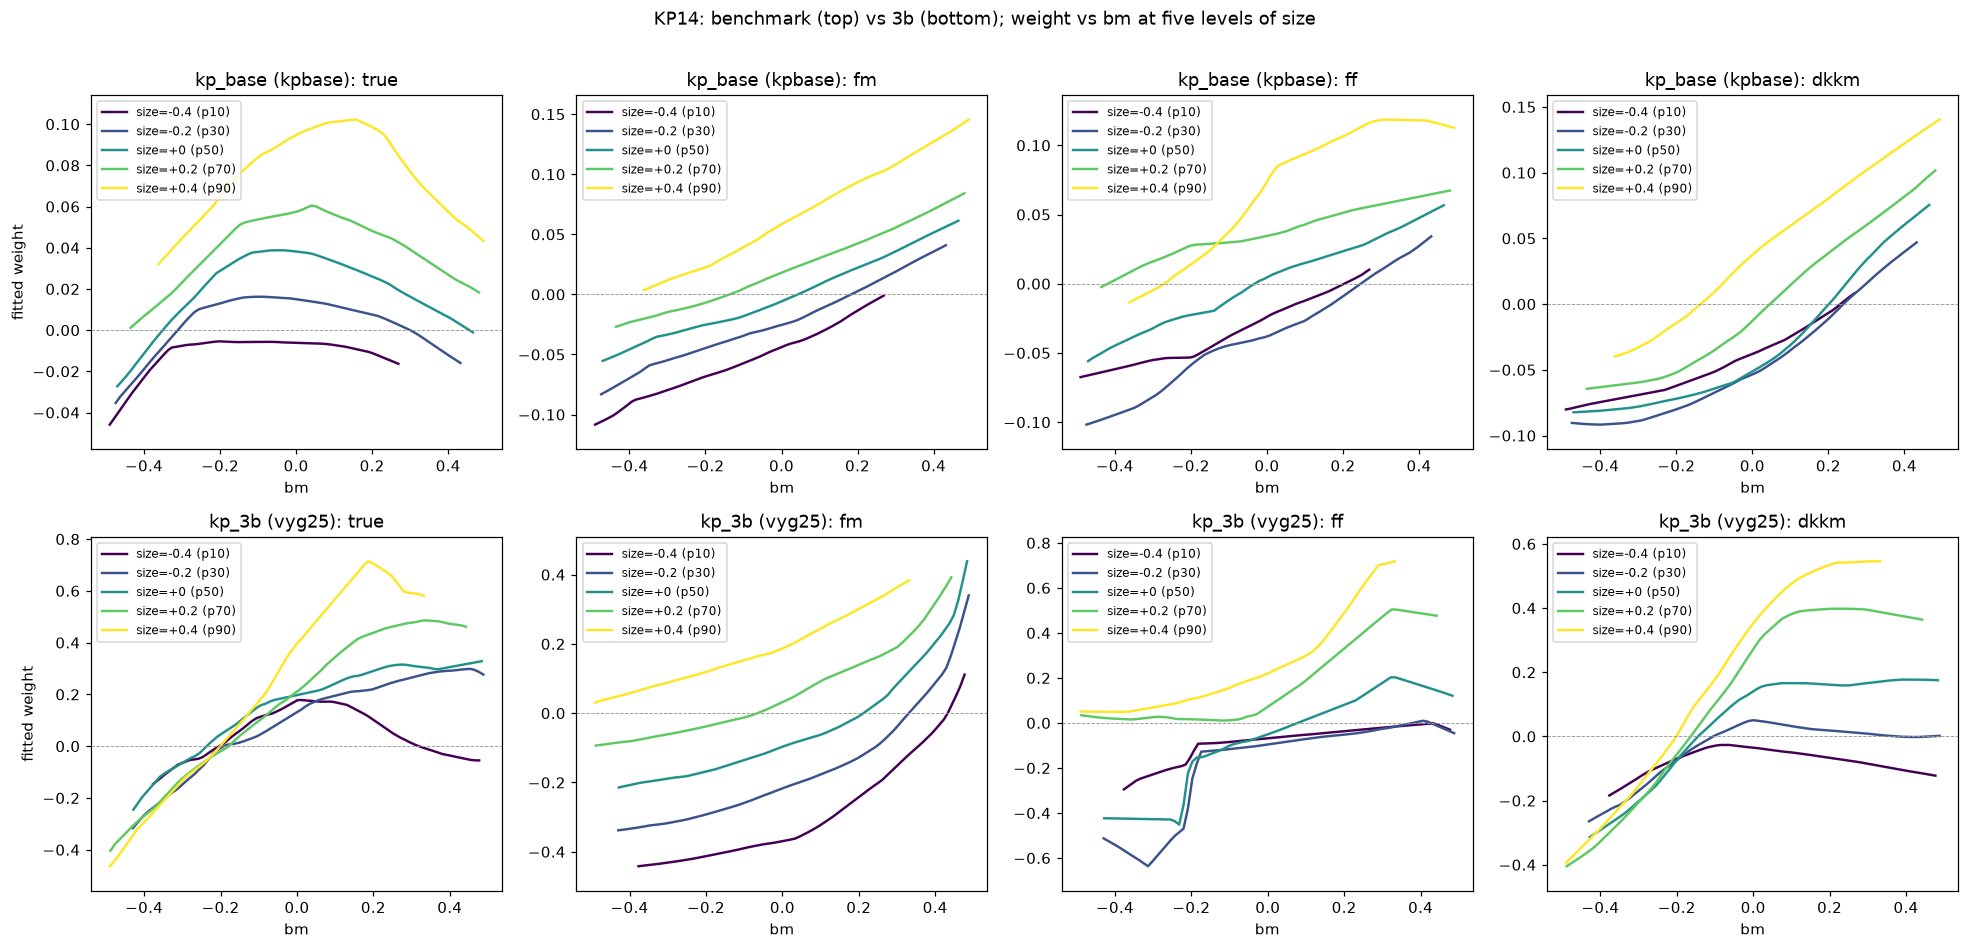
\includegraphics[width=\textwidth]{mlp_figures/compare_kp_vary_bm_fix_size.png}\caption{KP14: fitted weight against book-to-market at five levels of size (benchmark above, 3b below); panels: true SDF, Fama--MacBeth, Fama--French, DKKM; other characteristics at their mean.}\end{figure}
\begin{figure}[htbp]\centering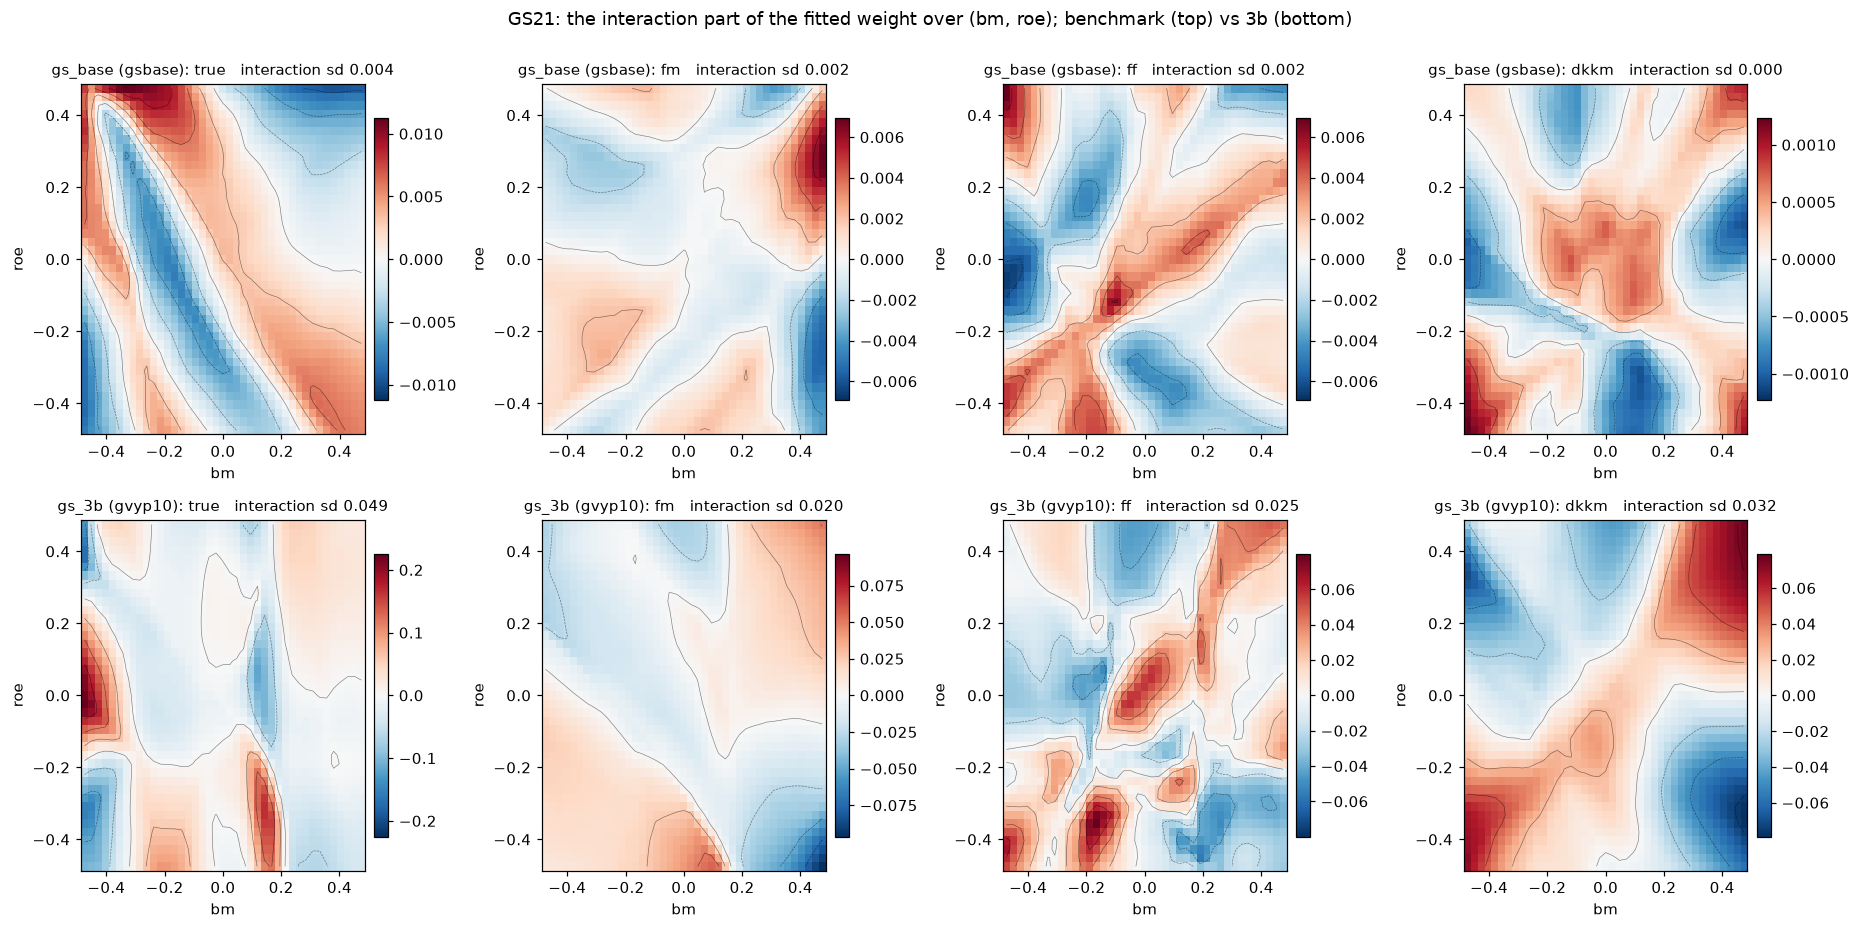
\includegraphics[width=\textwidth]{mlp_figures/interaction_gs_bmxroe.png}\caption{GS21: the interaction part of the fitted weight over profitability and book-to-market (benchmark above, 3b below); panels: true SDF, Fama--MacBeth, Fama--French, DKKM, each on its own colour scale, the interaction's sd in weight units in the title.}\end{figure}
\begin{figure}[htbp]\centering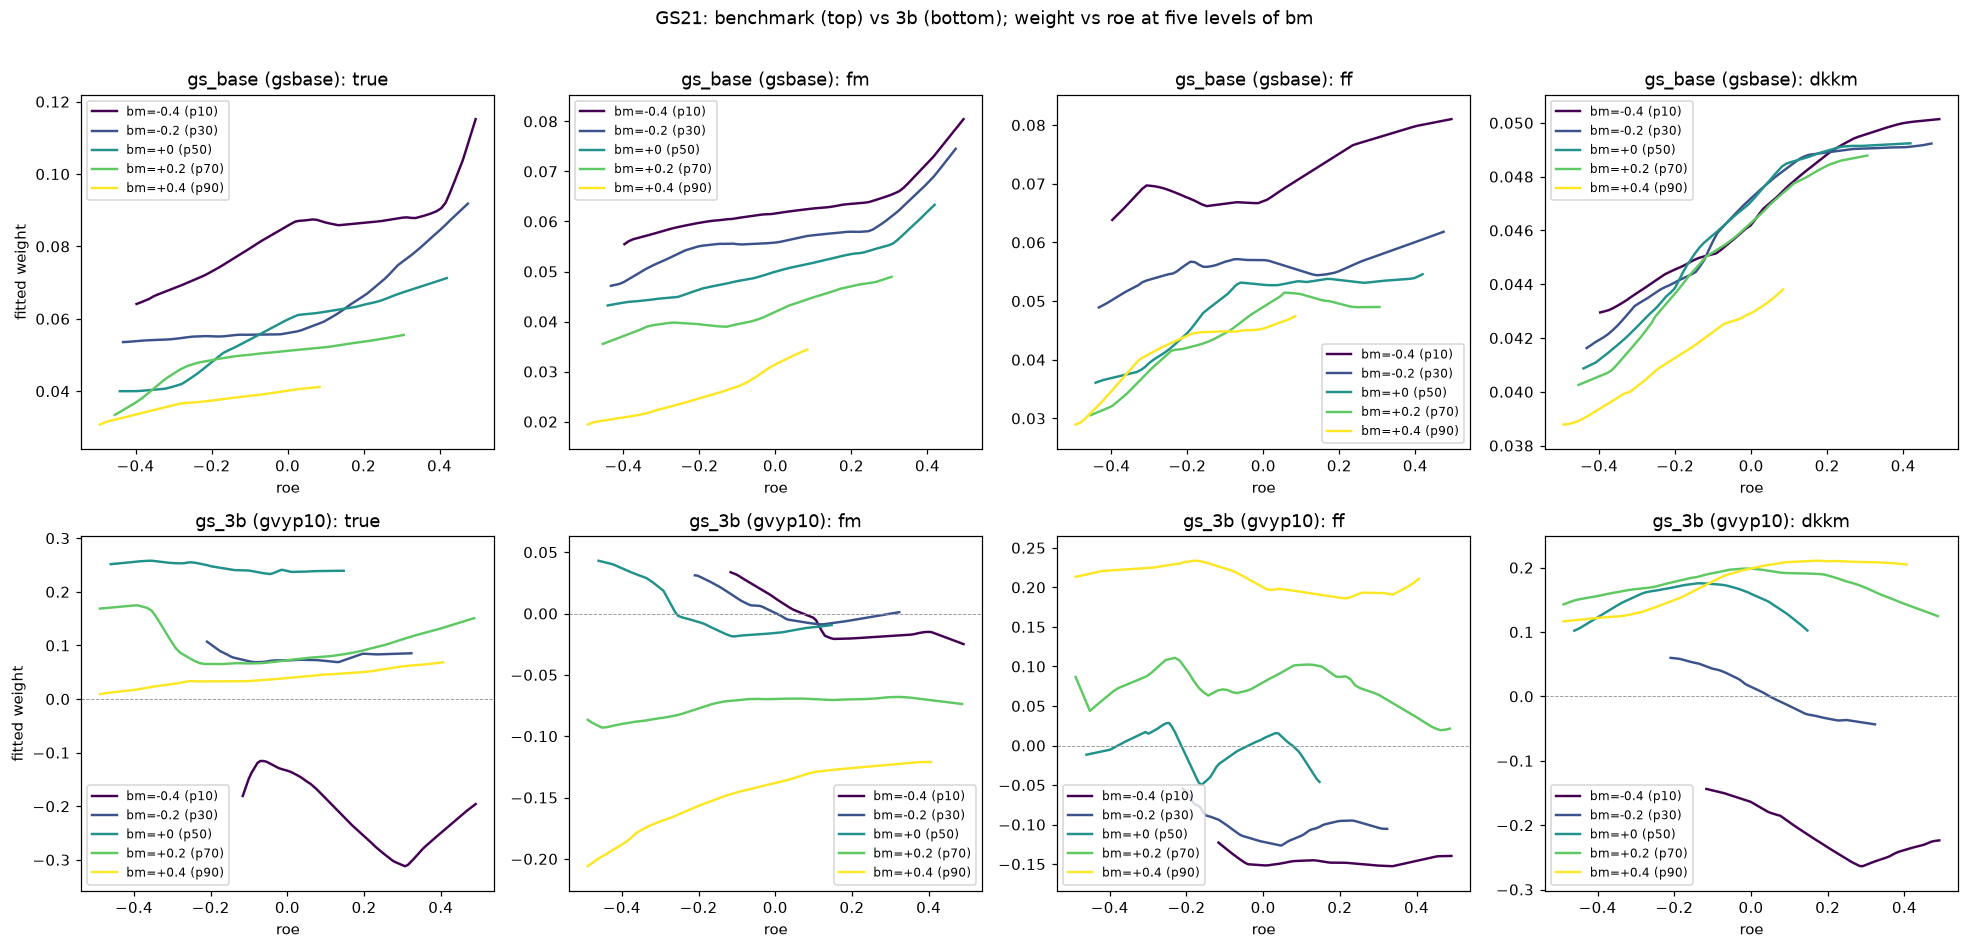
\includegraphics[width=\textwidth]{mlp_figures/compare_gs_vary_roe_fix_bm.png}\caption{GS21: fitted weight against profitability at five levels of book-to-market (benchmark above, 3b below); panels: true SDF, Fama--MacBeth, Fama--French, DKKM; other characteristics at their mean.}\end{figure}
\begin{figure}[htbp]\centering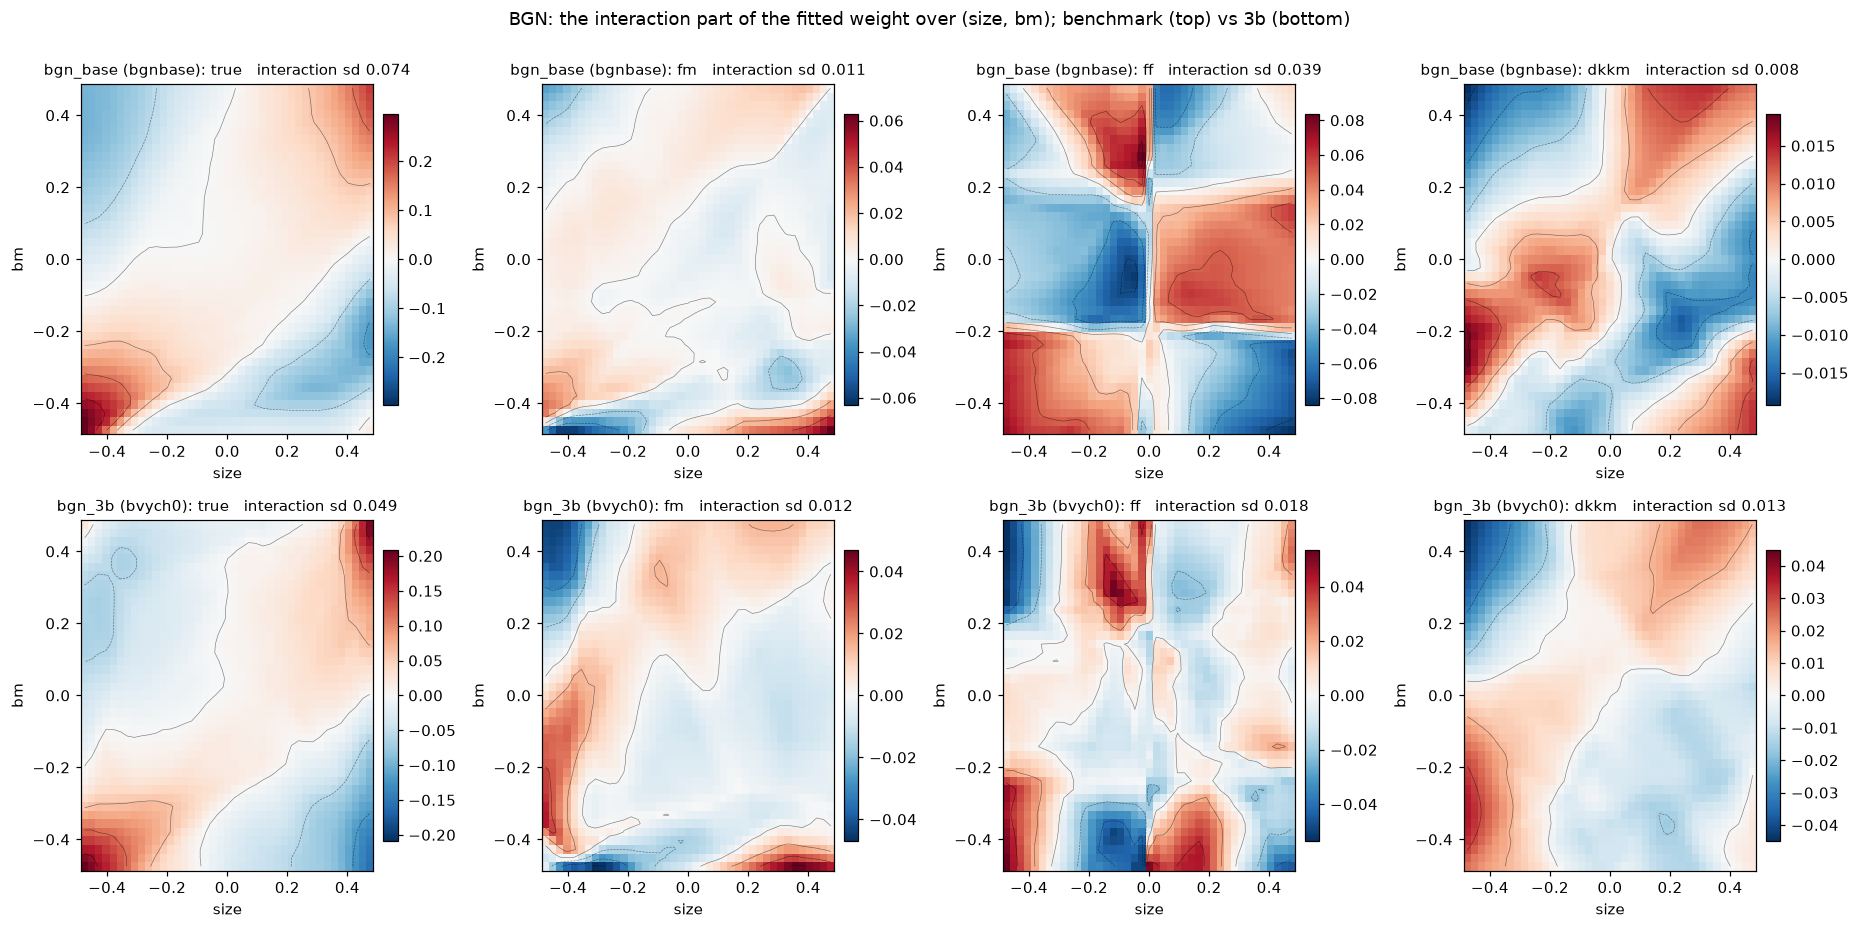
\includegraphics[width=\textwidth]{mlp_figures/interaction_bgn_sizexbm.png}\caption{BGN: the interaction part of the fitted weight over book-to-market and size (benchmark above, 3b below); panels: true SDF, Fama--MacBeth, Fama--French, DKKM, each on its own colour scale, the interaction's sd in weight units in the title.}\end{figure}
\begin{figure}[htbp]\centering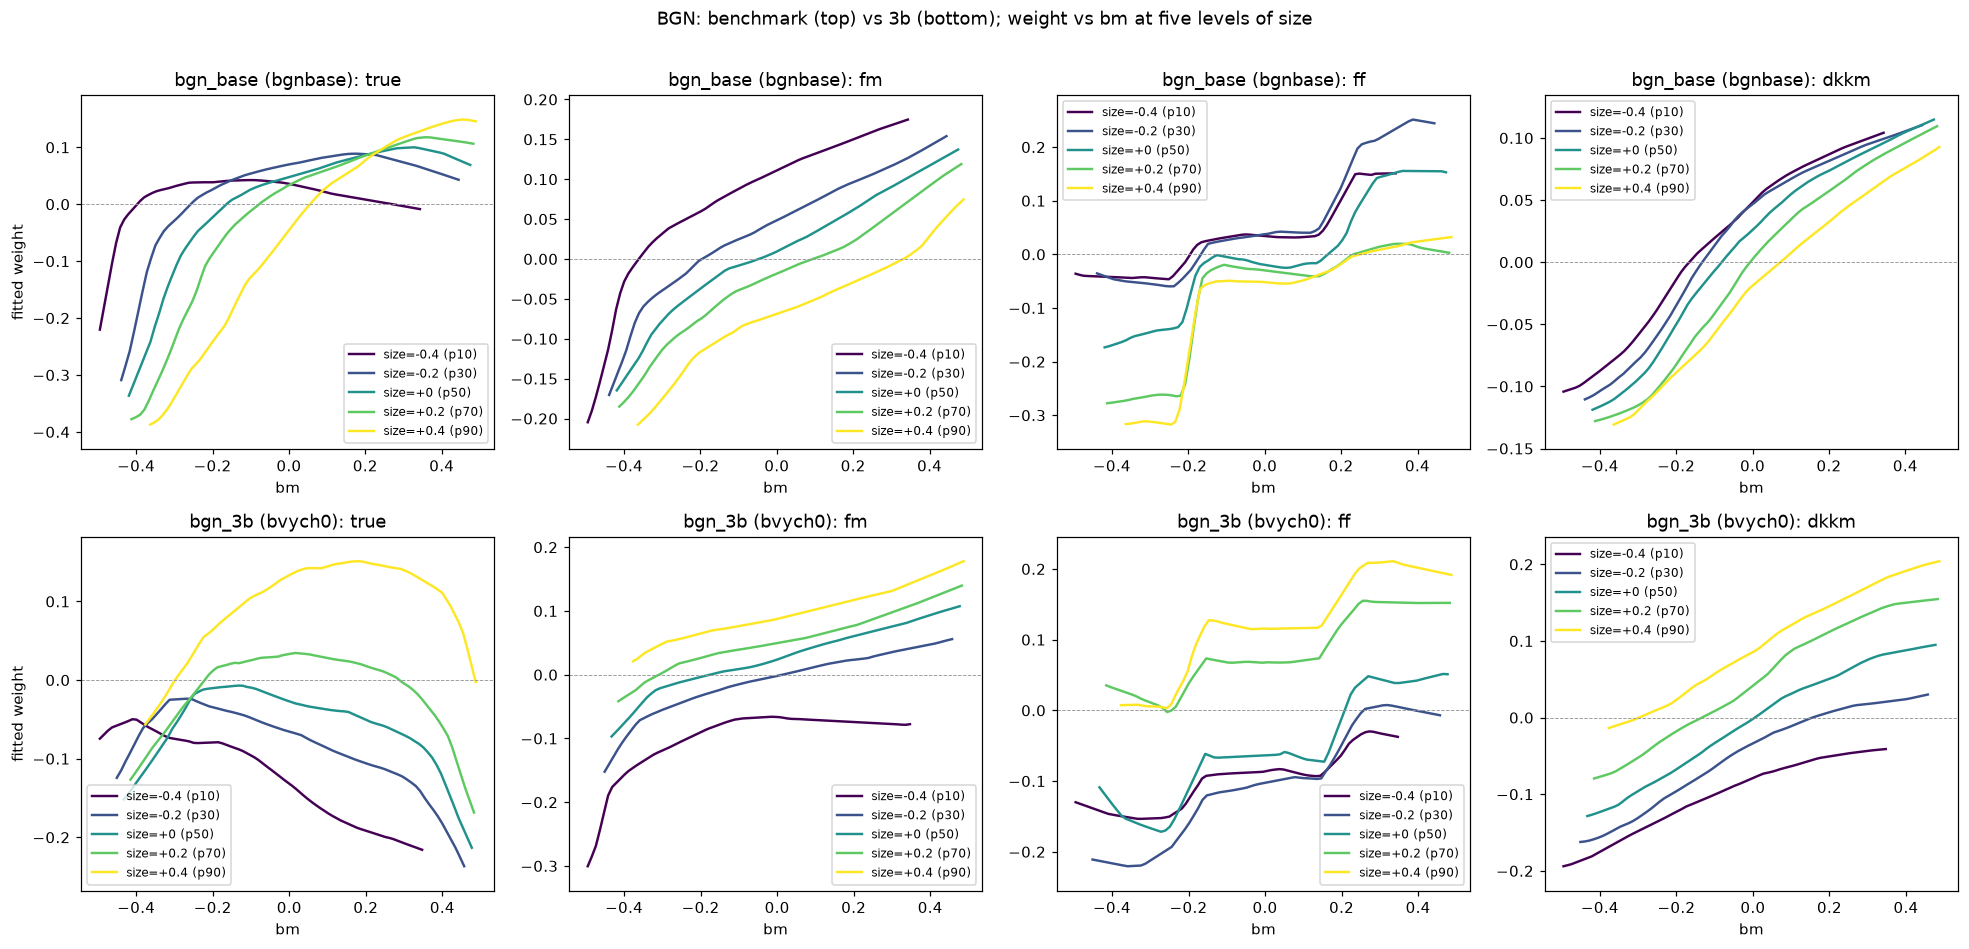
\includegraphics[width=\textwidth]{mlp_figures/compare_bgn_vary_bm_fix_size.png}\caption{BGN: fitted weight against book-to-market at five levels of size (benchmark above, 3b below); panels: true SDF, Fama--MacBeth, Fama--French, DKKM; other characteristics at their mean.}\end{figure}
